\section{Part 4: Kalman Filter in practice}

\begin{frame}{Part 4: Practical Guidelines for Kalman Filter Implementation}
		
		\textbf{Including:}
				
		\begin{itemize}
			\item Sensor fusion 
			\item Variable measurement uncertainty
                \item Treatment of missing measurements 
                \item Treatment of outliers
                \item Kalman Filter design process
                \begin{itemize}
                    \item Kalman Filter Initialization
                    \item KF Development Process
                \end{itemize}
		\end{itemize}
\end{frame}

\subsection{Sensor Fusion}
\begin{frame}{Sensor Fusion}
    Many practical systems are equipped with several complementary and sometimes interchangeable sensors measuring the same parameters, e.g., 
    \begin{itemize}
        \item A self-driving car has \textbf{Light Detection and Ranging (LiDAR)} and \textbf{radar} onboard. The LiDAR is much more precise than the radar. On the other hand, the radar measures velocity using the Doppler Effect, and its effective operational range is higher, especially in rain or fog conditions.
        \item The aircraft is equipped with Global Navigation Satellite System (GNSS) and Inertial Navigation System (INS) systems for navigation.
        \item Many surveillance systems include several radars for target tracking.
    \end{itemize}

    Using multiple sensors can significantly improve the state estimation precision in a process known as sensor fusion.

    \textcolor{blue}{Sensor fusion refers to combining the measurements from multiple sensors resulting in joint information having less uncertainty than any of the sensors individually.}
\end{frame}

%%%%%%%%%%%%%%%%%%%%%%%%%%%%%%%%%%%%%%%%%%%%%%%%%%%%%%
\subsubsection{Combining measurements in one dimension}
\begin{frame}{Combining measurements in one dimension}
    \begin{columns}
        \column{0.5\textwidth} 
        Consider two range measurements of the same target performed by two independent radars simultaneously. The SNR of the first radar measurement is higher (lower uncertainty) than the SNR of the second radar measurement. 
        \begin{figure}
            \centering
            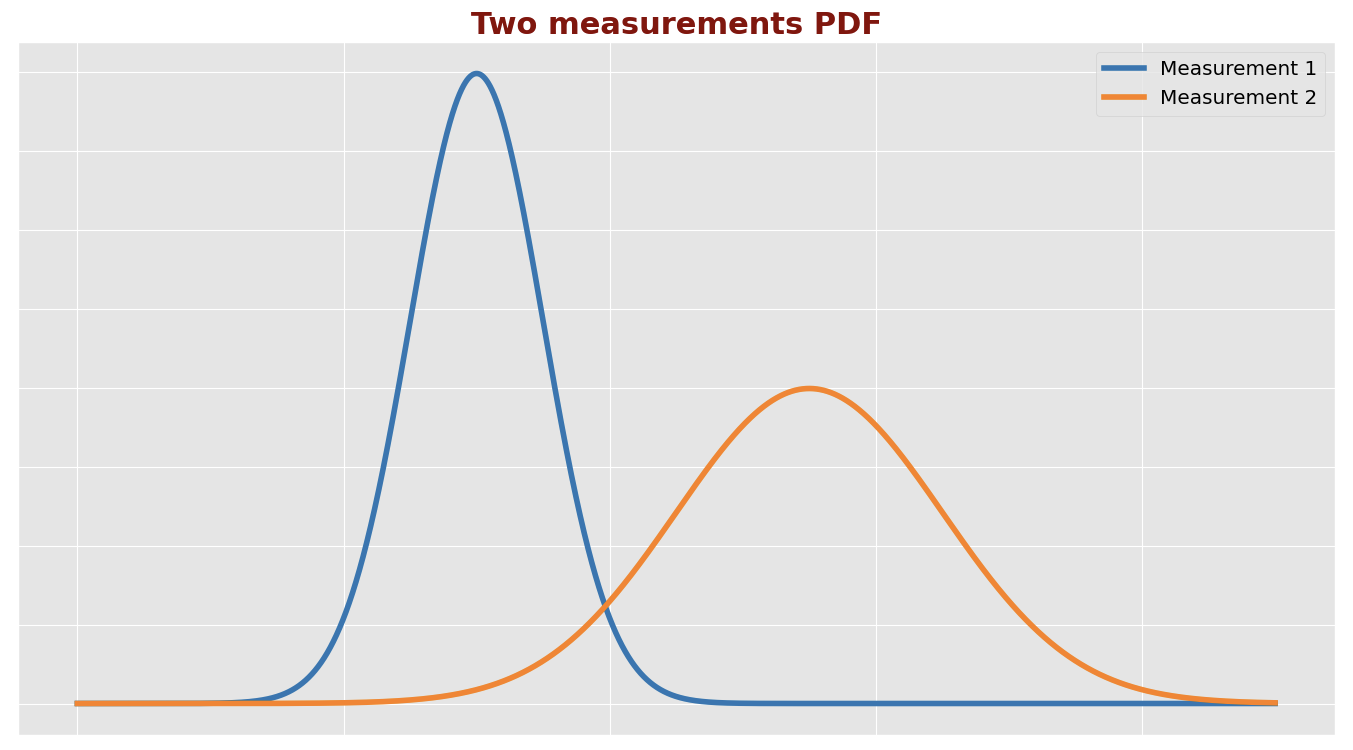
\includegraphics[width=0.5\linewidth]{Figures//Part4/TwoMeasurementsPDFs.png}
            \vspace{-10pt}
            \caption{PDF of measurements of both radars as normally distributed random variables.}
            \vspace{-10pt}
        \end{figure}

        Since the measurements are independent, the joint PDF is a product of two PDFs: 
        
        The variance \( \sigma^2_{12} \) is given by:
    \begin{equation*}
        \sigma^2_{12} = \left( \frac{1}{\sigma^2_1} + \frac{1}{\sigma^2_2} \right)^{-1}
    \end{equation*}
        The mean \( \mu_{12} \) is given by:
        \begin{equation*}
            \mu_{12} = \left( \frac{\mu_1}{\sigma^2_1} + \frac{\mu_2}{\sigma^2_2} \right) \sigma^2_{12}
        \end{equation*}
    
        \column{0.5\textwidth}

    \begin{itemize}
        \item Each measurement is weighted by the inverse of its variance. If the variance of the first measurement is lower than the variance of the second measurement ($\sigma^2_1 < \sigma^2_2$), then the weight of the first measurement is higher.
        \item That means the Gaussian PDFs product is closer to the measurement with lower
variance.
        \item The variance of the Gaussian PDFs product is always lower than the variance of each measurement separately. Even a measurement with a very high variance contributes to the overall precision. If $\sigma^2_2 = \infty$ then $\sigma^2_{12} = \sigma^2_1$.
    \end{itemize}
    \begin{figure}
        \centering
        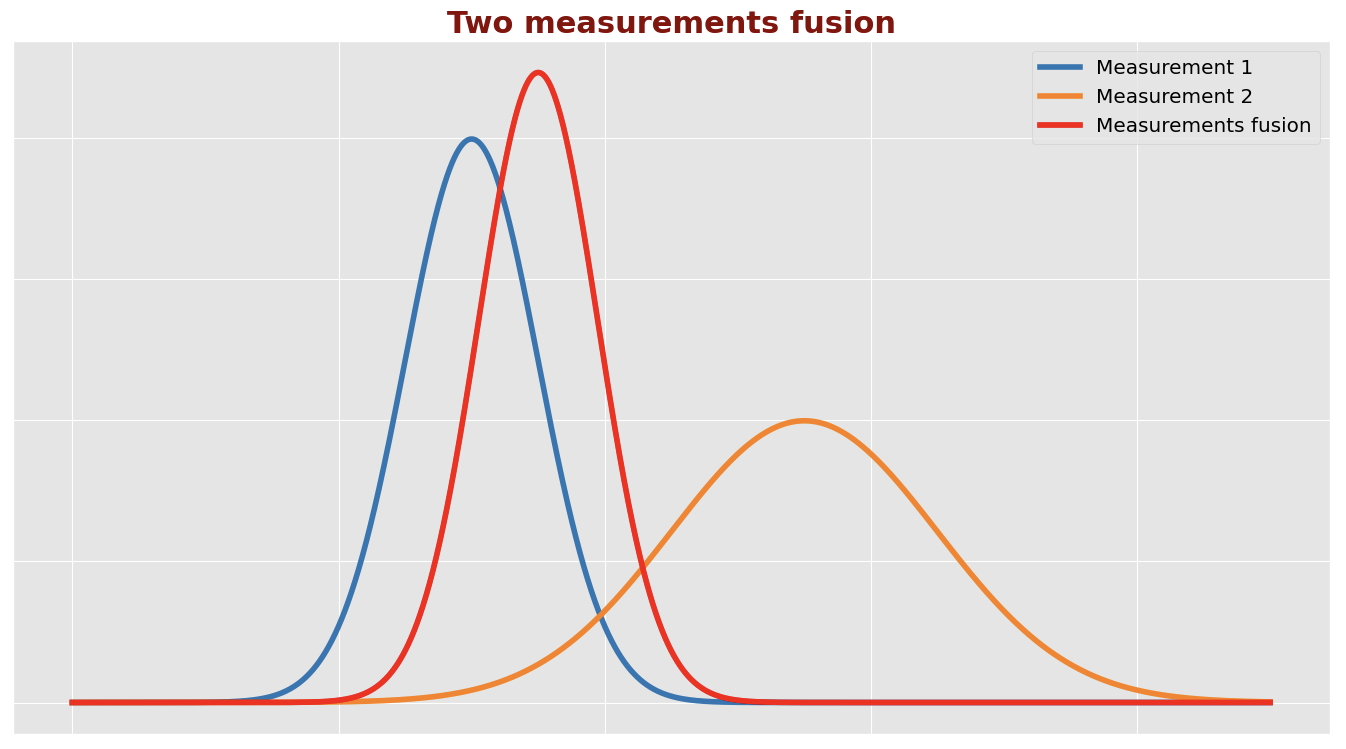
\includegraphics[width=0.5\linewidth]{Figures//Part4/TwoMeasurementsFusion.png}
        \vspace{-10pt}
        \caption{Joint PDF is closer to the measurement with a lower variance.}
        \vspace{-10pt}
    \end{figure}
    \end{columns}
\end{frame}


%%%%%%%%%%%%%%%%%%%%%%%%%%%%%%%%%%%%%%%%%%%%%%%%%%%%%%
\subsubsection{Combining $n$ measurements}
\begin{frame}{Combining $n$ measurements}
The product of univariate Gaussian PDFs results in a \( k \)-dimensional Gaussian PDF with the following properties:

The variance \( \sigma^2_{1 \cdots n} \) is given by:
\begin{equation*}
\sigma^2_{1 \cdots n} = \left( \frac{1}{\sigma^2_1} + \frac{1}{\sigma^2_2} + \cdots + \frac{1}{\sigma^2_n} \right)^{-1} = \left( \sum_{i=1}^{n} \frac{1}{\sigma^2_i} \right)^{-1}
\end{equation*}
Showing that every additional measurement minimizes the overall uncertainty.
\vspace{5pt}

The mean \( \mu_{1 \cdots n} \) is given by:
\begin{equation*}
\mu_{1 \cdots n} = \left( \sum_{i=1}^{n} \frac{\mu_i}{\sigma^2_i} \right) \sigma^2_{1 \cdots n}
\end{equation*}

\end{frame}

%%%%%%%%%%%%%%%%%%%%%%%%%%%%%%%%%%%%%%%%%%%%%%%%%%%%%%
\subsubsection{Combining measurements in $k$ dimensions}
\begin{frame}{Combining measurements in $k$ dimensions}
The multivariate \( k \)-dimensional normal distribution is given by:
\begin{equation*}
p(x) = \frac{1}{\sqrt{(2\pi)^k |\Sigma|}} \exp \left( -\frac{1}{2} (x - \mu)^T \Sigma^{-1} (x - \mu) \right)
\end{equation*}
where:
\begin{itemize}
    \item \( \mu \) is the mean vector
    \item \( \Sigma \) is the covariance matrix
\end{itemize}

\begin{columns}
    \column{0.5\textwidth}
    The product of \( n \) \( k \)-dimensional Gaussian PDFs is also a \( k \)-dimensional Gaussian PDF with the following properties:

\begin{equation*}
\Sigma^{-1}_{1 \cdots n} = \sum_{i=1}^{n} \Sigma^{-1}_i
\end{equation*}

\begin{equation*}
\mu_{1 \cdots n} = \Sigma \left( \sum_{i=1}^{n} \Sigma^{-1}_i \mu_i \right)
\end{equation*}
Like in the univariate Gaussian case, the mean of the product of the PDFs is the weighted mean of all PDFs, while the PDF with a lower variance has a higher weight. 
    \column{0.5\textwidth}
    Each PDF contributes to the joint PDF and reduces the joint PDF covariance.
    \begin{figure}
        \centering
        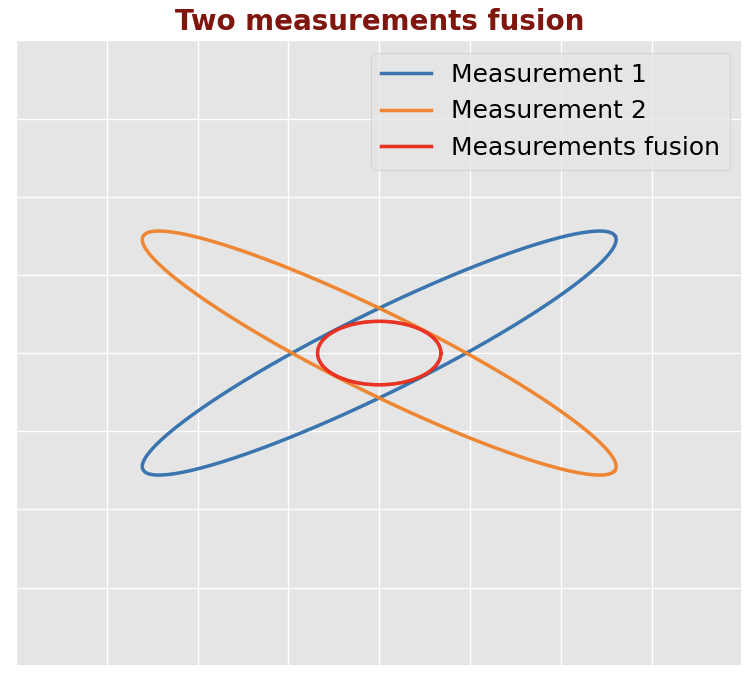
\includegraphics[width=0.5\linewidth]{Figures//Part4/Two2DMeasurementsFusion.png}
        \vspace{-10pt}
        \caption{Two 2D measurements fusion: The blue and orange ellipses represent the covariance of two measurements, and the red ellipse represents the covariance of the joint PDF.}
    \end{figure}

\end{columns}

\end{frame}


%%%%%%%%%%%%%%%%%%%%%%%%%%%%%%%%%%%%%%%%%%%%%%%%%%%%%%
\subsubsection{Sensor data fusion using Kalman filter}
\begin{frame}{Sensor data fusion using Kalman filter: Measurements fusion}
\begin{columns}
    \column{0.5\textwidth}
    Kalman filter is the most widespread algorithm for multisensor data fusion. We discuss two methods for multisensor data fusion using the Kalman filter, assuming identical sensors’ sample rates (for simplicity).

    \textbf{Method 1 – measurements fusion:} Measurement fusion is the most common sensor data fusion method. Typically it is used by a system that is equipped with several sensors.
    \begin{figure}
        \centering
        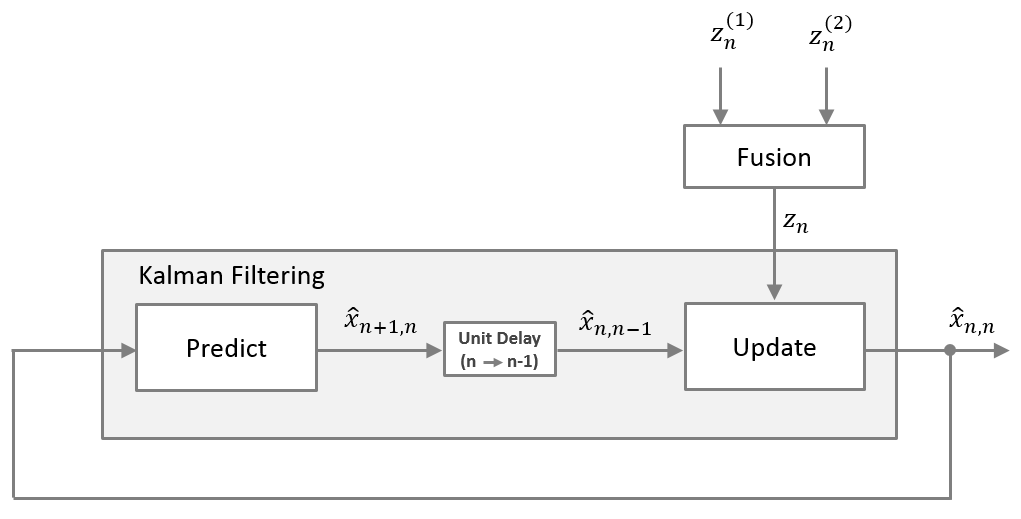
\includegraphics[width=0.9\linewidth]{Figures//Part4/TwoMeasurementsSensorFusion.png}
        \vspace{-10pt}
        \caption{Sensors measurements fusion}
        \vspace{-10pt}
    \end{figure}
        Two or more sensors provide measurements \( \bm{z}^{(1)}_n, \bm{z}^{(2)}_n, \ldots, \bm{z}^{(k)}_n \) with measurement covariance \( \bm{R}^{(1)}_n, \bm{R}^{(2)}_n, \ldots, \bm{R}^{(k)}_n \). Assuming normally distributed measurement PDFs, we can calculate a joint PDF, with parameters:


    \column{0.5\textwidth}
        \begin{equation*}
        \bm{R}^{-1}_n = \sum_{i=1}^{k} \bm{R}^{-1}_i
        \end{equation*}
        
        The unified measurement \( \bm{z}_n \) is given by:
        \begin{equation*}
        \bm{z}_n = \bm{R}_n \left( \sum_{i=1}^{k} \bm{R}^{(i)^{-1}}_n \bm{z}^{(i)}_n \right)
        \end{equation*}
        
        The conventional Kalman Filter receives the unified measurement \( (\bm{z}_n, \bm{R}_n) \).
        
        In the literature, you can also see that \( \bm{z}_n \) for two sensors is calculated as follows:
        \begin{equation*}
        \bm{z}_n = \bm{z}^{(1)}_n + \bm{R}^{(1)}_n \left( \bm{R}^{(1)}_n + \bm{R}^{(2)}_n \right)^{-1} \left( \bm{z}^{(2)}_n - \bm{z}^{(1)}_n \right)
        \end{equation*}
        
        \textcolor{blue}{It is identical to the Kalman Filter state update equation, which also calculates the fusion of two normally distributed PDFs – the measurement and the prior estimate uncertainty.}
        
        Second, it is computationally effective.
\end{columns}
\end{frame}


%%%%%%%%%%%%%%%%%%%%%%%%%%%%%%%%%%%%%%%%%%%%%%%%%%%%%%
\begin{frame}{Sensor data fusion using Kalman filter: State fusion}
\begin{columns}
    \column{0.5\textwidth}
    Some applications involve different sensor systems that perform the same task. For example, several geographically distributed radars can track the same target. Each radar creates a separate target track using the Kalman filter.

    \vspace{5pt}
    An external system can receive radars’ tracks and compute a unified track with higher location precision. \textbf{The state fusion method is also called the track-to-track fusion algorithm.}
    \begin{figure}
        \centering
        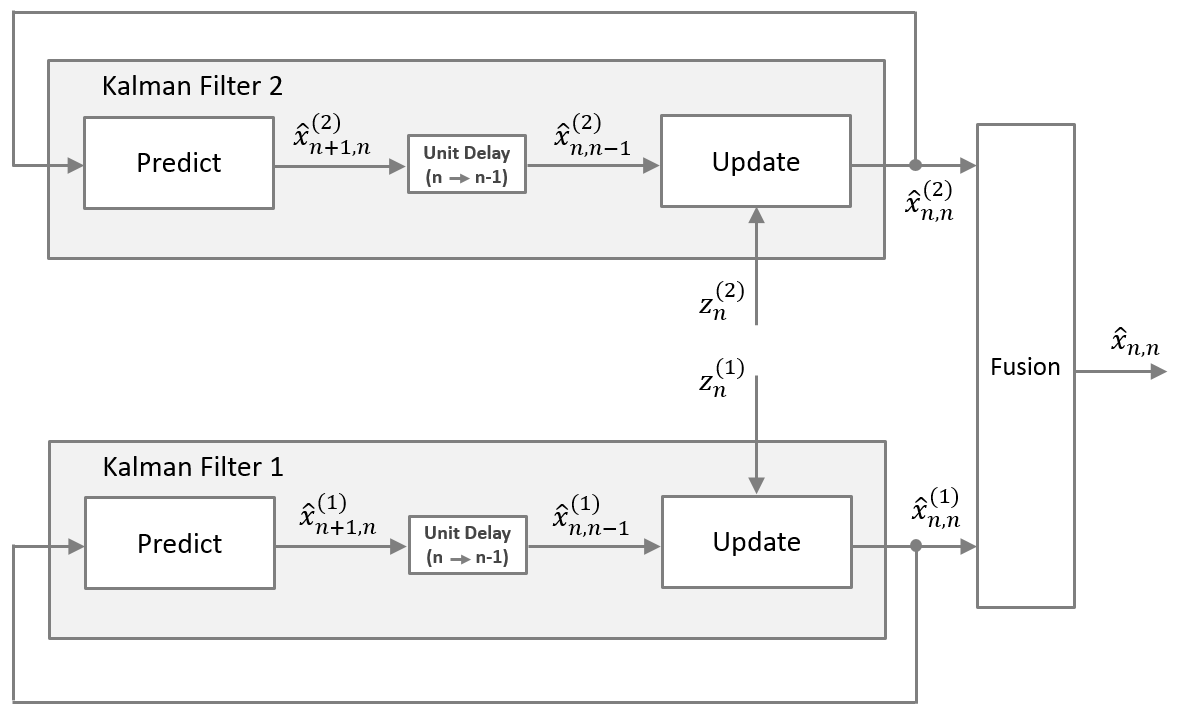
\includegraphics[width=0.9\linewidth]{Figures//Part3/Track2TrackFusion.png}
        \caption{State fusion or track-to-track fusion.}
    \end{figure}
    \column{0.5\textwidth}
    \textbf{State Fusion with Ignored Cross-Covariance: } When the cross-covariance between the two track estimates can be ignored, the state fusion involves a simple fusion of two random variables \( \hat{x}^{(1)}_{n,n} \) and \( \hat{x}^{(2)}_{n,n} \) with estimate uncertainties \( \bm{P}^{(1)}_{n,n} \) and \( \bm{P}^{(2)}_{n,n} \):

\begin{equation*}
\hat{x}_{n,n} = \hat{x}^{(1)}_{n,n} + \bm{P}^{(1)}_{n,n} \left( \bm{P}^{(1)}_{n,n} + \bm{P}^{(2)}_{n,n} \right)^{-1} \left( \hat{x}^{(2)}_{n,n} - \hat{x}^{(1)}_{n,n} \right)
\end{equation*}

The estimate covariance of the joint state \( \hat{x}_{n,n} \) is:

\begin{equation*}
\bm{P}^{-1}_{n,n} = \bm{P}^{(1)^{-1}}_{n,n} + \bm{P}^{(2)^{-1}}_{n,n}
\end{equation*}
textbf{State Fusion with Cross-Covariance:} The measurements from the two sensor tracks are not necessarily independent, as they can be correlated due to common process noise from the target dynamics. To avoid degradation in the target state estimates, these correlated estimation errors must be considered when combining the state estimates.
\end{columns}

\end{frame}



%%%%%%%%%%%%%%%%%%%%%%%%%%%%%%%%%%%%%%%%%%%%%%%%%%%%%%
\begin{frame}{Sensor data fusion using Kalman filter: State fusion}
The method for correlated state fusion was shown by Bar-Shalom~\cite{Chang_Track2TrackFusion}. The fused state is given by:
\begin{equation*}
\hat{x}_{n,n} = \hat{x}^{(1)}_{n,n} + \left( \bm{P}^{(1)}_{n,n} - \bm{P}^{(12)}_{n,n} \right) \left( \bm{P}^{(1)}_{n,n} + \bm{P}^{(2)}_{n,n} - \bm{P}^{(12)}_{n,n} - \bm{P}^{(21)}_{n,n} \right)^{-1} \left( \hat{x}^{(2)}_{n,n} - \hat{x}^{(1)}_{n,n} \right)
\end{equation*}

\(\bm{P}^{(12)}_{n,n} = \left( \bm{P}^{(21)}_{n,n} \right)^T\) is the cross-covariance matrix between \(\hat{x}^{(1)}_{n,n}\) and \(\hat{x}^{(2)}_{n,n}\). The cross-covariance matrix is given by:
\begin{equation*}
\bm{P}^{(12)}_{n,n} = \left( \bm{I} - \bm{K}^{(1)}_n \bm{H}^{(1)} \right) \bm{F} \bm{P}^{(12)}_{n,n-1} \bm{F}^T \left( \bm{I} - \bm{K}^{(2)}_n \bm{H}^{(2)} \right)^T + \left( \bm{I} - \bm{K}^{(1)}_n \bm{H}^{(1)} \right) \bm{G} \bm{Q} \bm{G}^T \left( \bm{I} - \bm{K}^{(2)}_n \bm{H}^{(2)} \right)^T
\end{equation*}
where:
\begin{itemize}
    \item \(\bm{K}\) is the Kalman Gain
    \item \(\bm{H}\) is the Observation Matrix
    \item \(\bm{F}\) is the State Transition Matrix
    \item \(\bm{Q}\) is the Process Noise Covariance Matrix
    \item \(\bm{G}\) is the Control Matrix
\end{itemize}

Bar-Shalom and Campo showed~\cite{BarShalom1986TheEO} that when this dependence is taken into account, the area of the uncertainty ellipse is reduced by 70\% instead of being cut by 50\% as would be the case if the independent noise assumption were correct.

\end{frame}



%%%%%%%%%%%%%%%%%%%%%%%%%%%%%%%%%%%%%%%%%%%%%%%%%%%%%%
\subsubsection{Multirate Kalman Filter}
\begin{frame}{Multirate Kalman Filter}

In many applications, the sensors’ sample rates are not identical. For example, assume two sensors with a sampling rate of $\Delta t$ and $3\Delta t$. The Kalman Filter update scheme is elaborated below.
\begin{figure}
    \centering
    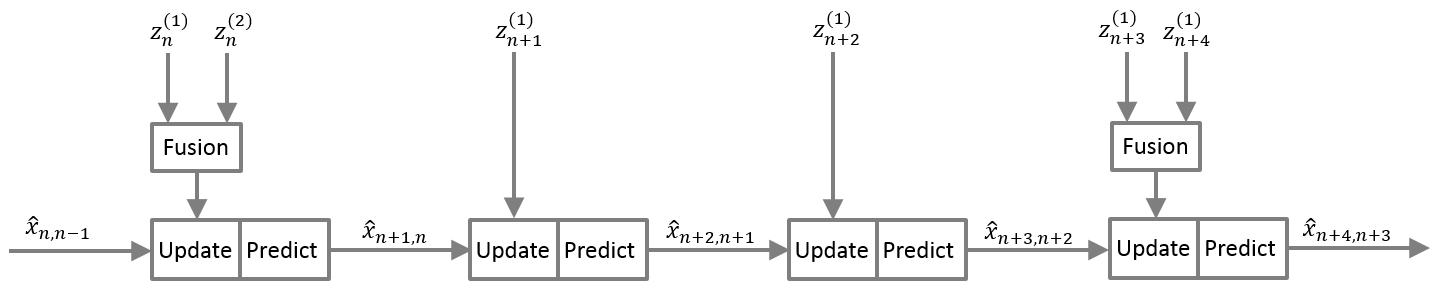
\includegraphics[width=0.9\linewidth]{Figures//Part4/MR_KF.png}
    \caption{Multirate Kalman Filter}
\end{figure}
The first sensor measurement updates the Kalman Filter state every $\Delta t$ period. Every
$3\Delta t$ period, the measurements of the first and the second sensors are combined.
\end{frame}



%%%%%%%%%%%%%%%%%%%%%%%%%%%%%%%%%%%%%%%%%%%%%%%%%%%%%%
\subsection{Variable Measurement Error}
\begin{frame}{Variable Measurement Error}
    \begin{itemize}
        \item In all examples, the measurement uncertainty is constant. For many measurement devices, the measurement uncertainty is a parameter given by the vendor. For example, the weight measurement accuracy of the scales or the power measurement accuracy of the power meter is a constant value.
        \item However, in many systems, the measurement uncertainty varies between successive measurements. For example, in a radar system, the range accuracy (standard deviation) is given by:
        \begin{equation*}
        \sigma_R = \frac{c}{2B \sqrt{\text{SNR}}}
        \end{equation*}
    where:
    \begin{itemize}
        \item \( \sigma_R \) is the range measurement error (standard deviation)
        \item \( c \) is the speed of light
        \item \( B \) is the signal bandwidth
        \item SNR is the signal-to-noise ratio
    \end{itemize}
    The radar range measurement variance is:
    \begin{equation*}
    r_n = \sigma^2_{R_n} = \frac{c^2}{4B^2 \text{SNR}_n}
    \end{equation*}
    
    We can see that the range measurement uncertainty depends on SNR. The SNR depends on many factors, such as interferences, target range, and perspective. For a radar system, the measurement uncertainty is not constant.

    \end{itemize}
\end{frame}



%%%%%%%%%%%%%%%%%%%%%%%%%%%%%%%%%%%%%%%%%%%%%%%%%%%%%%
\subsection{Treating missing measurements}
\begin{frame}{Treating missing measurements}
Sometimes the sensor measurements are lost due to noisy communication channels, interferences, equipment malfunctions, or other anomalies. In such cases, you can set the measurement to an arbitrary value while setting the measurement variance to infinity.

The Kalman Gain would be zero:
\[
\bm{K}_n = \frac{\bm{p}_{n,n-1}}{\bm{p}_{n,n-1} + \bm{r}_n} = \frac{\bm{p}_{n,n-1}}{\bm{p}_{n,n-1} + \infty} = 0
\]

The current state estimation \( \hat{x}_{n,n} \) would be equal to the prior estimate \( \hat{x}_{n,n-1} \):
\[
\hat{x}_{n,n} = \hat{x}_{n,n-1} + 0 (z_n - \hat{x}_{n,n-1}) = \hat{x}_{n,n-1}
\]

The current state estimation variance \( \bm{p}_{n,n} \) would be equal to the prior extrapolated state variance \( \bm{p}_{n,n-1} \):
\[
\bm{p}_{n,n} = (1 - 0) \bm{p}_{n,n-1} = \bm{p}_{n,n-1}
\]

In case of missing measurement, the extrapolated state variance \( \bm{p}_{n+1,n} \) would increase due to the process noise:
\[
\bm{p}_{n+1,n} = \bm{p}_{n,n} + \bm{q}_n = \bm{p}_{n,n-1} + \bm{q}_n
\]

Therefore, the missing measurement causes a temporary Kalman Filter divergence.
\end{frame}


%%%%%%%%%%%%%%%%%%%%%%%%%%%%%%%%%%%%%%%%%%%%%%%%%%%%%%
\subsection{Treating outliers: Identification and Treatment}
\begin{frame}{Treating outliers}
\begin{columns}
    \column{0.5\textwidth}
    Outliers are measurements outside an expected range or don’t follow an expected pattern. Outliers can result from noisy communication channels, interferences, equipment malfunctions, recording errors, or other anomalies, such as radar signal reflection from a bypassing aircraft.
    \begin{figure}
        \centering
        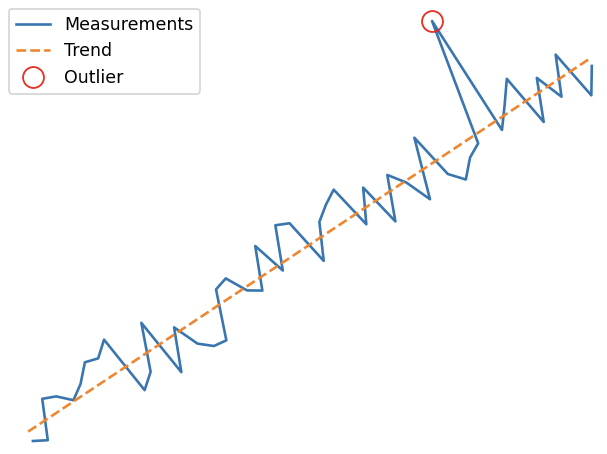
\includegraphics[width=0.6\linewidth]{Figures//Part4/Outliers.png}
        \vspace{-10pt}
        \caption{Outliers example}
    \end{figure}
    \textcolor{blue}{\textbf{Identifying Outliers:}} We can divide outliers into two main categories:
    
    \textbf{1. Unlikely or unusual measurements:} Sometimes you may decide that the measurement is unlikely based on your technical knowledge of the domain.
    
    \column{0.5\textwidth}
    \begin{itemize}
        \item If the vehicle speed measurement is 400km/h, you can decide that the measurement is an outlier since the car can’t travel at that speed.
        \item If the vehicle position measurement is far from the road, it is likely an outlier.
        \item The water temperature above $100^o$C is an outlier.
    \end{itemize}
    \textbf{2. High statistical distance:} Assume a system that estimates the vehicle speed using the Kalman Filter. The prior estimate of the speed (prediction) $\hat{x}{n,n-1}$ is 100km/h, and the measured speed $z_n$ is 120km/h. The difference between the predicted and measured values is 20km/h. \textbf{Is it an outlier?}
    \begin{itemize}
        \item \textit{Mahalanobis distance} is needed to answer this: The Mahalanobis distance is a measure of the distance between a point $P$ and a distribution $D$ or between two random variables, introduced by P. C. Mahalanobis in 1936.
    \end{itemize}
    
\end{columns}
\end{frame}

%%%%%%%%%%%%%%%%%%%%%%%%%%%%%%%%%%%%%%%%%%%%%%%%%%%%%%
\begin{frame}{Treating outliers}
\begin{columns}
    \column{0.5\textwidth}
    \begin{itemize}
        \item In a single dimension, the Mahalanobis distance is given by:
        \[
        d_M = \sqrt{\frac{(\hat{x}_{n,n-1} - z_n)^2}{p_{n,n-1}}}
        \]
        where:
        \begin{itemize}
            \item \( \hat{x}_{n,n-1} \) is the prior estimate
            \item \( p_{n,n-1} \) is the prior estimate variance
            \item \( z_n \) is the measurement
        \end{itemize}
        \item For vehicle speed estimation example; if $p_{n,n-1} = 150 \text{km}^2/\text{h}^2$:
        \begin{figure}
            \centering
            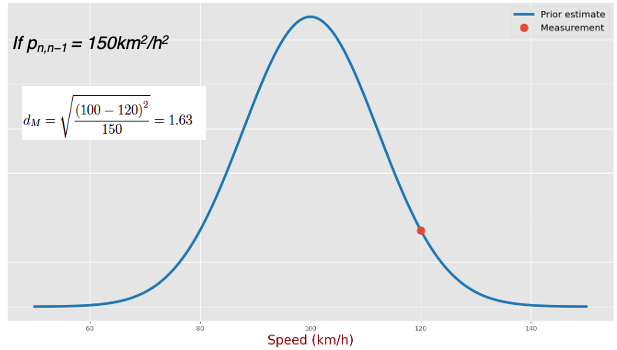
\includegraphics[width=0.7\linewidth]{Figures//Part3/LowMahalanobisDistrance.png}
            \vspace{-10pt}
            \caption{Low Mahalanobis Distance.}
            \vspace{-10pt}
        \end{figure}
        \item if $p_{n,n-1} = 10 \text{km}^2/\text{h}^2$:
        \end{itemize}    
    \column{0.5\textwidth}
    \begin{itemize}
        \item 
        \begin{figure}[!t]
            \centering
            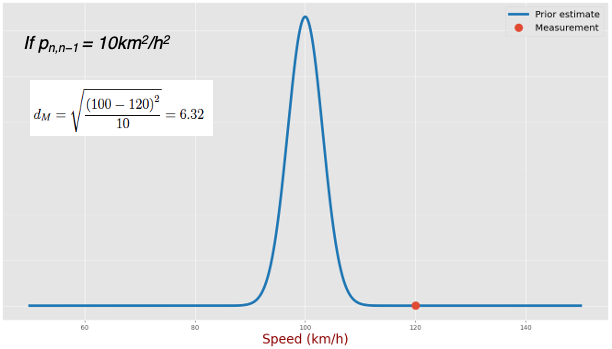
\includegraphics[width=0.7\linewidth]{Figures//Part4/HighMahalanobisDistance.png}
            \vspace{-10pt}
            \caption{High Mahalanobis Distance.}
            \vspace{-5pt}
        \end{figure}
        \item In the first case, the measurement is not an outlier since the distance of 1.63 standard deviations is reasonable. In the second case, the measurement is definitely an outlier.

        
        \item A Kalman Filter designer should define the Mahalanobis distance threshold based on the domain technical knowledge. Usually, it varies between 3 and 5.
        
        \item For a multivariate Kalman Filter, the $d_M$ is:
        \[
        d_M = \sqrt{(\hat{\bm{x}}_{n,n-1} - \bm{z}_n)^T \bm{P}_{n,n-1}^{-1} (\hat{\bm{x}}_{n,n-1} - \bm{z}_n)}
        \]
        \vspace{-10pt}
        \begin{itemize}
            \item \( \hat{\bm{x}}_{n,n-1} \) is the prior estimate
            \item \( \bm{P}_{n,n-1} \) is the prior estimate covariance matrix
            \item \( \bm{z}_n \) is the measurement vector
        \end{itemize}
    \end{itemize}
\end{columns}
\end{frame}



%%%%%%%%%%%%%%%%%%%%%%%%%%%%%%%%%%%%%%%%%%%%%%%%%%%%%%
\begin{frame}{Treating outliers}
\begin{columns}
    \column{0.5\textwidth}
    \textcolor{blue}{\textbf{Impact of Outliers:}}
    \begin{itemize}
        \item The impact of an outlier depends on the variance of the outlier. Let us continue with the example of vehicle speed estimation. The prior estimate of the speed (prediction) $\hat{x}{n,n-1}$ is 100km/h, and the measured speed $z_n$ is 120km/h. The calculated Mahalanobis distance for $p_{n,n-1} = 10 \text{km}^2/\text{h}^2$ is $d_M = 6.32$.
        \item The distance between the prior estimate and the measurement is 6.32 standard deviations; therefore, the measurement is an outlier.
        
        \item Let us take a look at the measurement uncertainty. The radar velocity measurement accuracy is given by:
        \[
        \sigma_V = \frac{\lambda B}{2 \sqrt{2 \text{SNR}}}
        \]
        \vspace{-5pt}
        \begin{itemize}
            \item \( \sigma_V \) is the velocity measurement error (standard deviation)
            \item \( \lambda \) is the signal wavelength
            \item \( B \) is the signal bandwidth
        \end{itemize}
    \end{itemize}
    \column{0.5\textwidth}
    \begin{itemize}
        \item The radar velocity measurement variance is:
        \[
        r_n = \sigma^2_{V_n} = \frac{\lambda^2 B^2}{8 \text{SNR}_n}
        \]
        \item Assume a noisy measurement with a low SNR that yields \( \sigma_{V_n} = 30 \text{ km/h} \).
        \begin{figure}
            \centering
            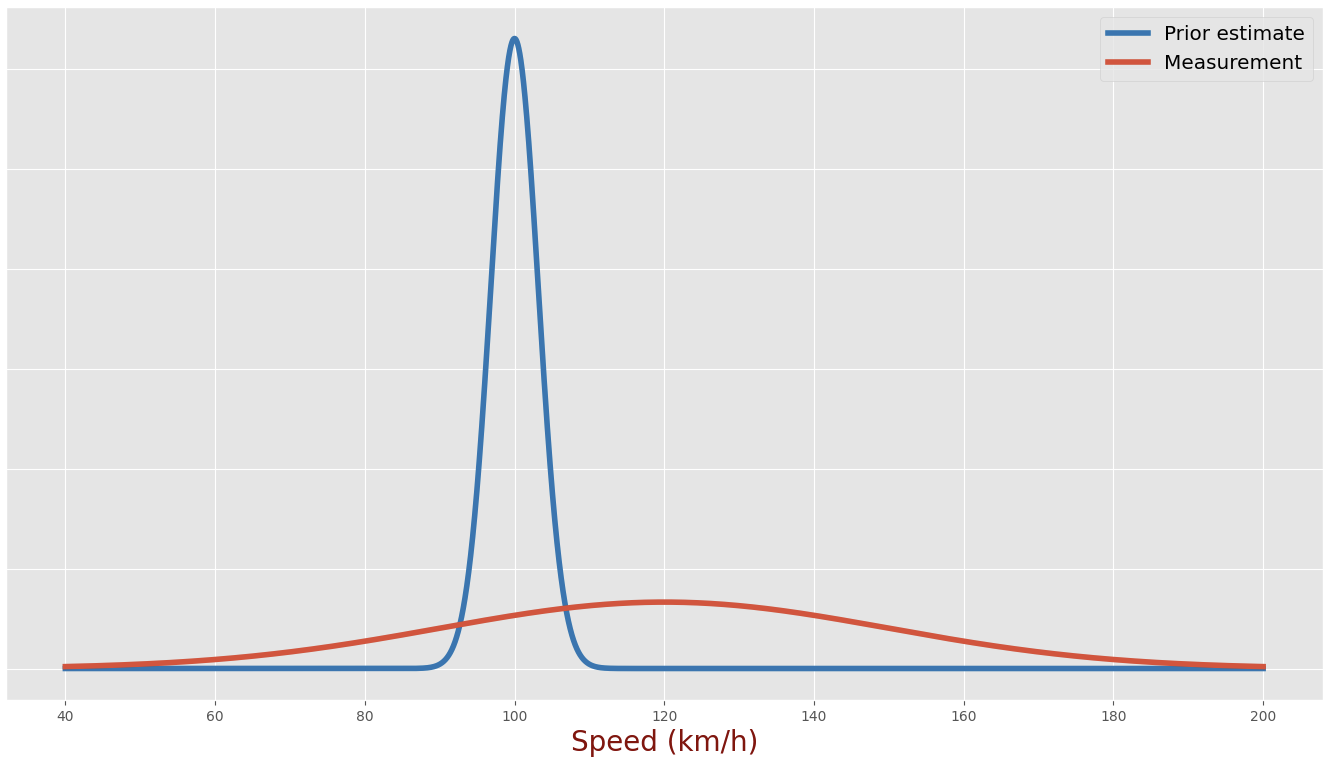
\includegraphics[width=0.35\linewidth]{Figures//Part4/AbnormalMeasurementwithHighUncertainty.png}
            \vspace{-10pt}
            \caption{Abnormal measurement with high uncertainty}
            \vspace{-10pt}
        \end{figure}
        \item The Kalman Gain is given by:
        \[
        \bm{K}_n = \frac{\bm{p}_{n,n-1}}{\bm{p}_{n,n-1} + \bm{r}_n} = \frac{10}{10 + 30^2} = 0.01
        \]

        \item The state update equation is:
        \begin{align*}
            \hat{x}_{n,n} &= \hat{x}_{n,n-1} + 0.01 (z_n - \hat{x}_{n,n-1}) \\ &= 0.99 \hat{x}_{n,n-1} + 0.01 z_n
        \end{align*}
        \item The Kalman Gain is very low; therefore, the impact of the noisy measurement with high uncertainty is very low.

    \end{itemize}
\end{columns}
\end{frame}



%%%%%%%%%%%%%%%%%%%%%%%%%%%%%%%%%%%%%%%%%%%%%%%%%%%%%%
\begin{frame}{Treating outliers}
\begin{columns}
    \column{0.5\textwidth}
    \begin{itemize}
        \item Now assume an outlier measurement with high SNR that yields \( \sigma_{V_n} = 2 \text{ km/h} \). Such a measurement can be caused by an anomaly.
        \begin{figure}
            \centering
            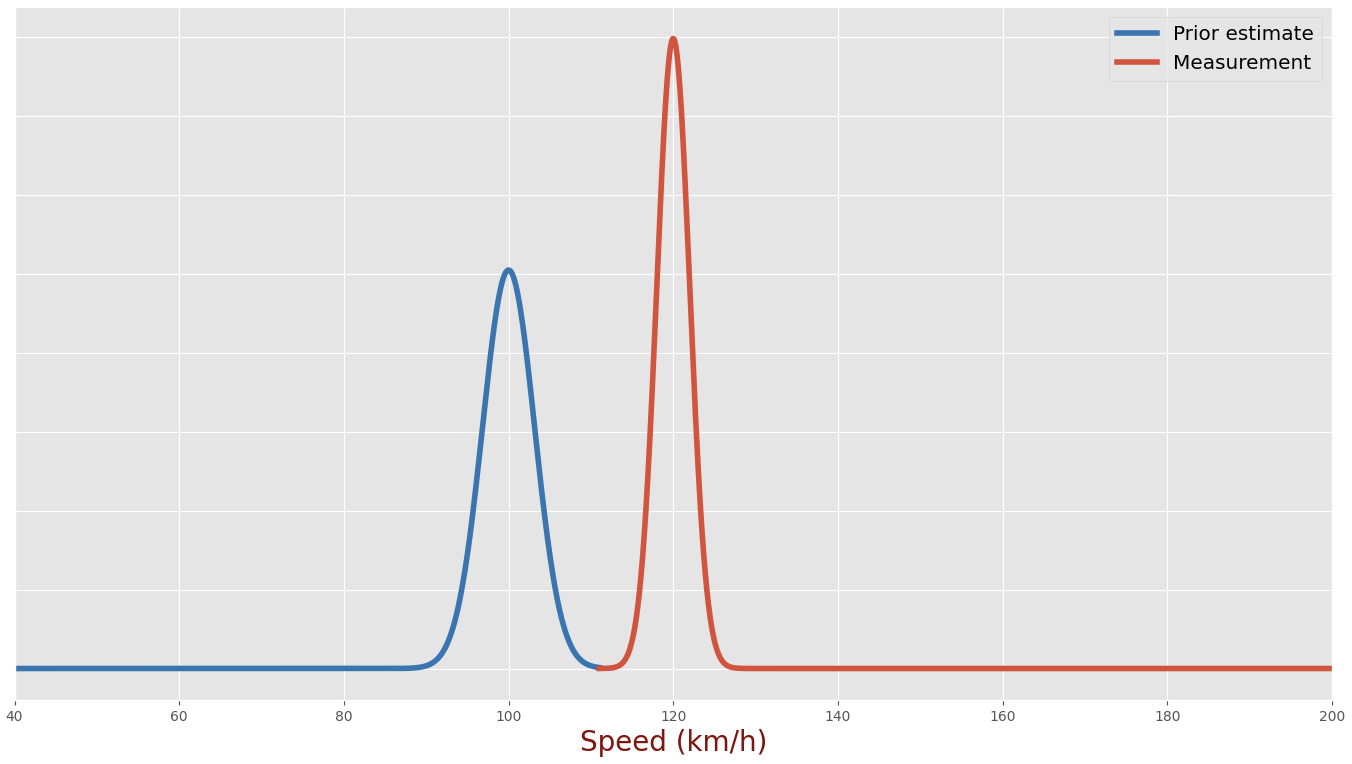
\includegraphics[width=0.5\linewidth]{Figures//Part4/AbnormalMeasurementwithLowUncertainty.png}
            \vspace{-10pt}
            \caption{Abnormal measurement with low uncertainty}
            \vspace{-10pt}
        \end{figure}
        \item The Kalman Gain is given by:
        \[
        \bm{K}_n = \frac{\bm{p}_{n,n-1}}{\bm{p}_{n,n-1} + \bm{r}_n} = \frac{10}{10 + 2^2} = 0.71
        \]

        \item The state update equation is:
        \begin{align*}
            \hat{x}_{n,n} &= \hat{x}_{n,n-1} + 0.71 (z_n - \hat{x}_{n,n-1}) \\ &= 0.29 \hat{x}_{n,n-1} + 0.71 z_n
        \end{align*}
        \item The Kalman Gain is very low; therefore, Kalman Gain is high; therefore, the impact of the abnormal measurement with low uncertainty is very high.
    \end{itemize}

    \column{0.5\textwidth}
    \textcolor{blue}{\textbf{Treating Outliers:}}
    \begin{itemize}
        \item A high-impact outlier influences long-term filter stability. It influences the current estimation and the following estimations as following estimations are based on the measurements and past estimations.
        \item For an outlier with a high Mahalanobis distance, eliminate the outlier and treat it as a missing measurement.

        \item If the outlier is unlikely or unusual, but the Mahalanobis distance is low, consider changing the outlier value to a reasonable value. E.g., when estimating the water temperature, set a temperature bound to $0^o$C and to $100^o$C. If the measurement temperature is $101^o$C, change it to $100^o$C.
        \item The outlier treatment algorithm includes the following steps:
        \begin{itemize}
            \item Identify an outlier by calculating the Mahalanobis Distance or based on the domain knowledge.
            \item Estimate the outlier impact.
            \item Eliminate the outlier or change its value to a lower or upper bound.
        \end{itemize}

        \end{itemize}
\end{columns}
\end{frame}



%%%%%%%%%%%%%%%%%%%%%%%%%%%%%%%%%%%%%%%%%%%%%%%%%%%%%%
\subsection{Kalman Filter Initialization}
\begin{frame}{Kalman Filter Initialization}

\begin{columns}
    \column{0.5\textwidth}
    The Kalman Filter must be initiated with a prior estimation $\hat{x}_{0,0}$ and initialization covariance ${P}_{0,0}$.
    \vspace{5pt}
    
    \textbf{Linear KF:} In Example~9--vehicle location estimation, with true vehicle location at the time $t = 0$ as $x = 300, y = -425$, what if we change initialization as
    \vspace{-5pt}
    \[
    \hat{x}_{0,0} =
    \begin{bmatrix}
    0 \\
    0 \\
    0 \\
    0 \\
    0 \\
    0 \\
    0
    \end{bmatrix} \rightarrow = \begin{bmatrix}
    303 \\
    0 \\
    0 \\
    -428 \\
    0 \\
    0 \\
    0
    \end{bmatrix}
    \]
    i.e., we initiate the Kalman Filter close to the actual vehicle position. 

    \vspace{5pt}
    Since our initial state vector was a guess, we set a very high estimate uncertainty. Now to see the effect of initialization, we must reduce the estimate uncertainty. The high estimate uncertainty results in a high Kalman Gain by giving a high weight to the measurement.
    
    \column{0.5\textwidth}
    \[\bm{P}_{0,0}=
\begin{bmatrix}
50 & 0 & 0 & 0 & 0 & 0 \\
0 & 50 & 0 & 0 & 0 & 0 \\
0 & 0 & 50 & 0 & 0 & 0 \\
0 & 0 & 0 & 50 & 0 & 0 \\
0 & 0 & 0 & 0 & 50 & 0 \\
0 & 0 & 0 & 0 & 0 & 50
\end{bmatrix}
\]
i.e., reduce to 50 from 500.
\begin{figure}
    \centering
    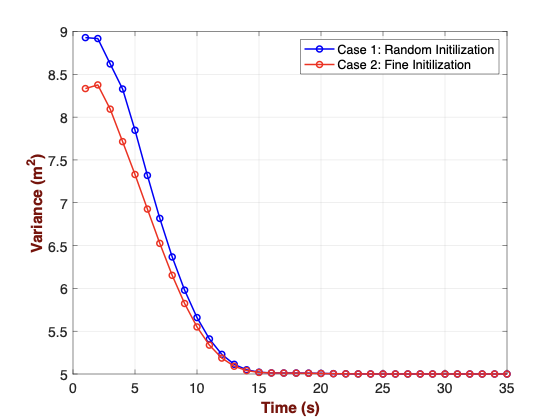
\includegraphics[width=0.7\linewidth]{Figures//Part4/Ex9_InitializationAspects.png}
    \vspace{-10pt}
    \caption{LKF uncertainty: rough vs. fine initiation.}
    \vspace{-10pt}
\end{figure}

We can see a lower uncertainty of the fine initialization. The KF converges faster if
we initiate it with meaningful values.
\end{columns}

\texttt{\tiny{[Code: Non-linear KF/Ex11\_InitializationAspects.m]}}
\end{frame}



%%%%%%%%%%%%%%%%%%%%%%%%%%%%%%%%%%%%%%%%%%%%%%%%%%%%%%
\begin{frame}{Kalman Filter Initialization}
\begin{columns}
    \column{0.5\textwidth}
    \textbf{Non-linear KF initialization:} Example~11--vehicle location estimation using radar. If the EKF is initiated close to the true position, the EKF converges quickly and accurately tracks the target.

    \[
\bm{x}_{0,0} =
\begin{bmatrix}
100 \\
0 \\
0 \\
-100 \\
0 \\
0
\end{bmatrix} \rightarrow = \bm{x}_{0,0} =
\begin{bmatrix}
100 \\
0 \\
0 \\
0 \\
0 \\
0
\end{bmatrix}
\]

\[
\bm{P}_{0,0} =
\begin{bmatrix}
500 & 0 & 0 & 0 & 0 & 0 \\
0 & 500 & 0 & 0 & 0 & 0 \\
0 & 0 & 500 & 0 & 0 & 0 \\
0 & 0 & 0 & 500 & 0 & 0 \\
0 & 0 & 0 & 0 & 500 & 0 \\
0 & 0 & 0 & 0 & 0 & 500
\end{bmatrix}
\]

    \column{0.5\textwidth}
    \begin{figure}
        \centering
        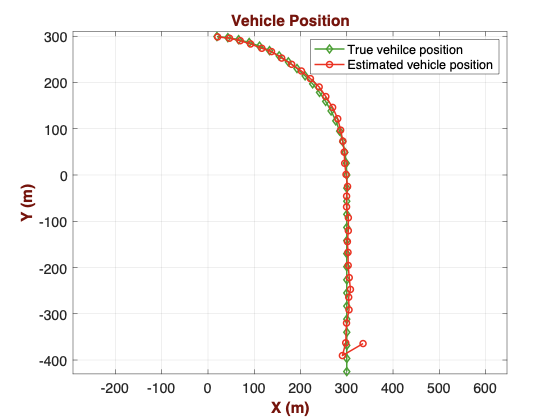
\includegraphics[width=0.6\linewidth]{Figures//Part4/Ex11_InitializationAspects_Fine.png}
        \vspace{-5pt}
    \end{figure}
    If the initialization point is moved further, the EKF provides wrong estimations. After some time, it converges and tracks the target.
    \begin{figure}
        \centering
        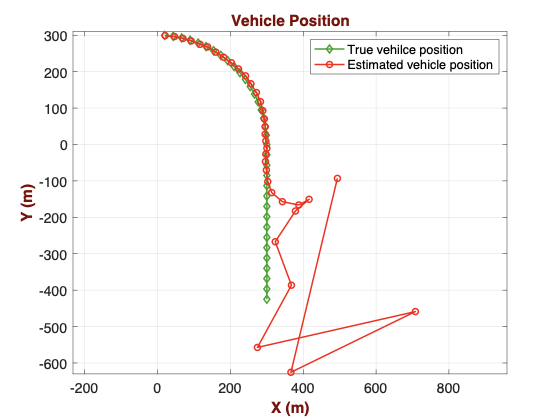
\includegraphics[width=0.6\linewidth]{Figures//Part4/Ex11_InitializationAspects_Bad.png}
        \vspace{-5pt}
    \end{figure}
    Unlike the LKF, the non-linear Kalman Filter requires fine initiation; otherwise, it wouldn’t be able to provide satisfactory results.
\end{columns}
\end{frame}



%%%%%%%%%%%%%%%%%%%%%%%%%%%%%%%%%%%%%%%%%%%%%%%%%%%%%%
\begin{frame}{KF initialization techniques}
\begin{itemize}
    \item There is no generic initialization technique or method. It depends on the system. 
    \item For example, the radar search process provides coarse target measurement used as initialization for the tracker.
    
    \item For other systems, an educated guess is sufficient for KF initialization.

    \item You can also use the \textbf{first measurement as initialization data} and start the estimation process with the second measurement.
\end{itemize}
\end{frame}


%%%%%%%%%%%%%%%%%%%%%%%%%%%%%%%%%%%%%%%%%%%%%%%%%%%%%%
\subsection{KF Development Process}
\begin{frame}{KF Development Process}

    The Kalman Filter development process includes four phases:
    \begin{itemize}
        \item Kalman Filter Design
        \item Simulation
        \item Performance Examination
        \item Parameters Tuning
    \end{itemize}
\begin{figure}
    \centering
    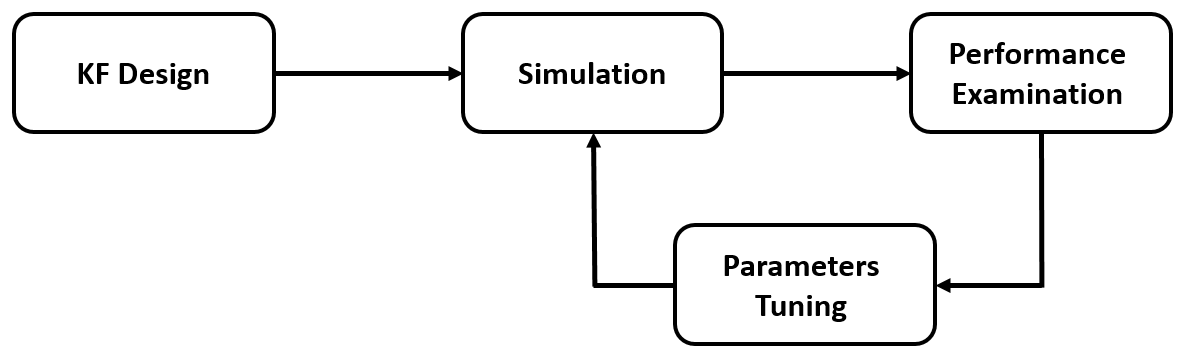
\includegraphics[width=0.6\linewidth]{Figures//Part4/KFDesignProcess.png}
    \caption{KF Design Process}
\end{figure}


\end{frame}


%%%%%%%%%%%%%%%%%%%%%%%%%%%%%%%%%%%%%%%%%%%%%%%%%%%%%%
\subsubsection{Kalman Filter Design}
\begin{frame}{KF Development Process: Follow 6-Steps of Kalman Filter Design}
\begin{columns}
    \column{0.5\textwidth}
\textbf{Step 1: Define the System Dynamic Model.}
\begin{itemize}
    \item Lucky if you know your system’s Dynamic Model (state extrapolation equation).
    \item Otherwise, write down the differential equations that govern your system (the state space representation), as:
    \vspace{-5pt}
    \begin{align*}
    \dot{\bm{x}}(t) &= \bm{A} \bm{x}(t) + \bm{B} \bm{u}(t) \\
    \bm{y}(t) &= \bm{C} \bm{x}(t) + \bm{D} \bm{u}(t)
    \end{align*}
    \vspace{-20pt}
    \item Solve the equations to determine the state extrapolation equation.
    \vspace{-5pt}
    \[
    \hat{\bm{x}}_{n+1,n} = \bm{F} \hat{\bm{x}}_{n,n} + \bm{G} \hat{\bm{u}}_{n,n} 
    \]
    \vspace{-20pt}
    \item For a non-linear system, the differential equation is in the form of:
    \vspace{-5pt}
    \[
    \dot{\bm{x}}(t) = \bm{g}(\bm{x}(t))
    \]
    \vspace{-20pt}
    \item Solve the differential equation to determine the state extrapolation equation:
    \vspace{-5pt}
    \[
    \hat{\bm{x}}_{n+1,n} = \bm{f}(\hat{\bm{x}}_{n,n}) + \bm{G} \hat{\bm{u}}_{n,n} 
    \]
    \vspace{-20pt}
    \item If the differential equation cannot be solved, perform the numerical integration of:
        \vspace{-5pt}
        \[
        \bm{f}(\hat{\bm{x}}_{n,n}) = \hat{\bm{x}}_{n,n} + \int_{t_n}^{t_{n+1}} \bm{g}(\bm{x}(t)) \, dt
        \]
\end{itemize}

    \column{0.5\textwidth}
    \vspace{-5pt}
    \textbf{Step 2: Define the measurement equation.}
    \begin{itemize}
        \item For LKF: $\bm{z}_n = \bm{H} \bm{x}_n$
        \item For EKF: $\bm{z}_n = \bm{h}(\bm{x}_n)$
    \end{itemize}

\textbf{Step 3: Process Noise error sources:}
\begin{itemize}
    \item Write down a list of all the error sources.
    \item Define the Process Noise matrix \( Q \) based on uncorrelated error sources (white noise).
    \item The correlated noise sources must be a part of the Dynamic Model.
\end{itemize}

\textbf{Step 4: Decide the KF initialization method:}
\begin{itemize}
    \item Initialization method is system-dependent; it can be an educated guess, a coarse or first measurement.
    \item Decide initialization covariance \( \bm{P}_{0,0} \).
\end{itemize}

\textbf{Step 5: Add treatment for missing measurements.}

\textbf{Step 6: Decide outliers treatment method:}
\begin{itemize}
    \item Which measurement should be considered an outlier and how to treat it?
\end{itemize}
\end{columns}
\end{frame}


%%%%%%%%%%%%%%%%%%%%%%%%%%%%%%%%%%%%%%%%%%%%%%%%%%%%%%
\subsubsection{Simulation}
\begin{frame}{KF Development Process: Simulation}
\begin{columns}
    \column{0.5\textwidth}
    Simulation is a critical phase of the Kalman Filter development process. It allows to observe the filter performance in a controlled environment. The simulation is a computer program that contains the following modules:
    \begin{figure}
        \centering
        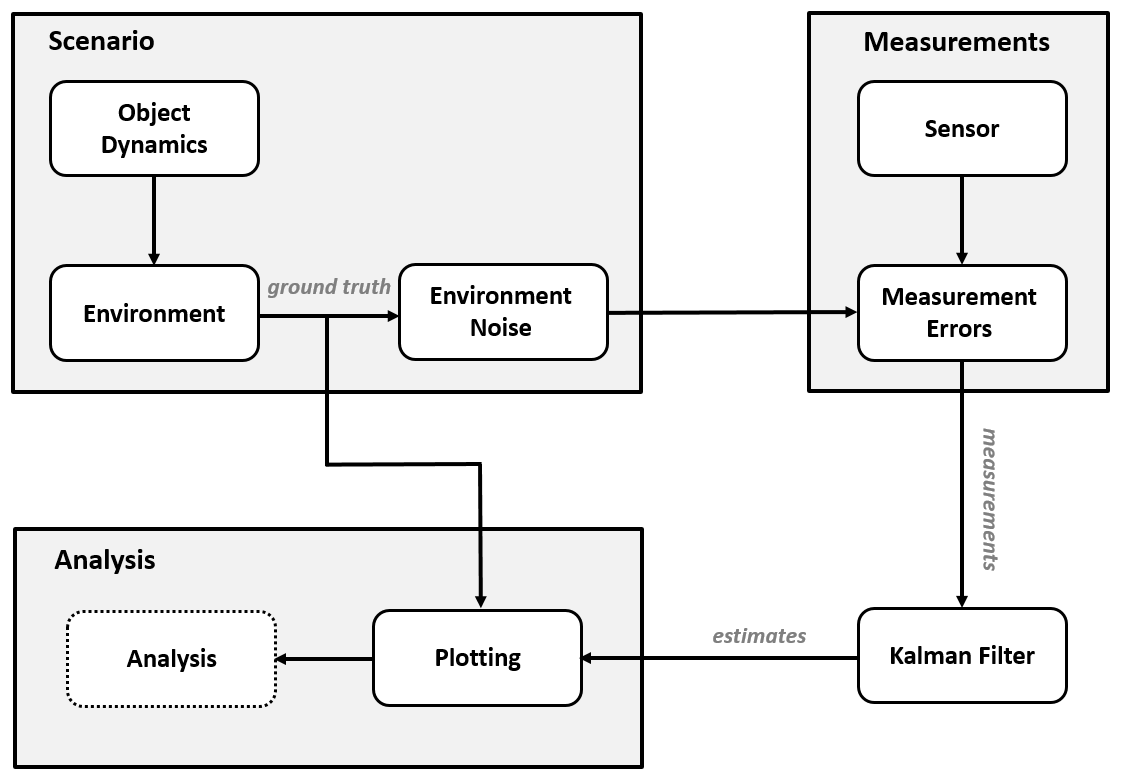
\includegraphics[width=0.7\linewidth]{Figures//Part4/KFSimulationFlow.png}
        \vspace{-10pt}
        \caption{KF Simulation Flow}
        \vspace{-10pt}
    \end{figure}
    \textbf{Scenario Module:} Simulating the real-world
    \begin{itemize}
        \item \textbf{Object dynamics} module generates different dynamics scenarios of the object of interest.
        \begin{itemize}
            \item For example, the vehicle trajectory, the pendulum position, or the heating liquid temperature.
            \item It shall include possible extreme conditions, like sharp target maneuvers.
        \end{itemize}
        \item 
    \end{itemize}
    \column{0.5\textwidth}
    \begin{itemize}
        \item \textbf{Environment} module simulates the environmental influence on the target dynamics, like air turbulence influence on the aircraft, the icy road influence on the vehicle, and the air-conditioner influence on the liquid temperature.

        \item \textbf{Generated scenario (or output):} 
        \begin{itemize}
            \item The generated scenario is a true state vector or the \textbf{ground truth}.
            \item The environment noise module adds noise to the ground truth - for example, an aircraft radar cross-section fluctuations, radio interferences, etc.
        \end{itemize}
    \end{itemize}
    \textbf{Measurements Module:} sensor measurements as input to Kalman Filter.
    \begin{itemize}
        \item For simple sensors like scales with a measurement uncertainty $\sigma$, generate a normally distributed random noise with std. $\sigma$, and add it to the generated scenario.
    \end{itemize}
\end{columns}
\end{frame}


%%%%%%%%%%%%%%%%%%%%%%%%%%%%%%%%%%%%%%%%%%%%%%%%%%%%%%
%\subsubsection{Simulation}
\begin{frame}{KF Development Process: Simulation}
    \begin{itemize}
        \item For EKF, the ground truth should be transformed into the sensor coordinates. For example, the vehicle position coordinates are X and Y while the sensor coordinates are range ($r$) and the bearing angle ($\theta$). Then the range noise and the angle noise should be added to the transformed coordinates.
        \item More sophisticated sensors require simulation of the sensor system to simulate phenomena like clock drift, imperfections due to sampling, and other system-specific aspects like beam broadening in radar.
    \end{itemize}

    \textbf{KF Module:} Same as KF design process.

    \textbf{Analysis:} Visualization of results as
    \begin{itemize}
        \item Estimates vs. measurements vs. ground truth.
        \item If possible, add estimation confidence intervals or confidence ellipses to the plot.
        \item Estimation uncertainty vs. time
        \item Kalman Gain vs. time
    \end{itemize}
\end{frame}


%%%%%%%%%%%%%%%%%%%%%%%%%%%%%%%%%%%%%%%%%%%%%%%%%%%%%%
\subsubsection{Performance Examination}
\begin{frame}{KF Development Process: Performance Examination}
\begin{columns}
    \column{0.5\textwidth}
    \begin{itemize}
        \item Before examining the KF performance, you should define the acceptable (reasonable) performance criteria. Don’t expect low errors if your sensor is not accurate or environmental noise is too high.
        \begin{itemize}
            \item The Root Mean Square (RMS) error between the ground truth and estimates.
            \item The RMS error between the ground truth and predictions.
            \item The maximum error between the ground truth and estimates.
            \item The maximum error between the ground truth and predictions.
            \item The filter convergence time.
            \item Prediction and estimation uncertainties.
            \item The confidence levels.
        \end{itemize}
    \item If the KF errors are too high, examine your dynamic model. You can increase the process noise ($\bm{Q}$) value. However, improving the dynamic model is a better approach.    
    \end{itemize}



    \column{0.5\textwidth}
\begin{itemize}
    \item Examine the filter convergence. The Kalman Gain should constantly decrease until it reaches a certain floor level. As a result, the uncertainty of the estimates should
also decrease. If the convergence time is too high, examine the influence of the KF initialization on the convergence time. Find methods for finer initialization values. You can also decrease the process noise ($\bm{Q}$) value, but make sure it doesn’t increase the errors.
\item Consider the results of Example~8.
\vspace{-5pt}
\begin{figure}
    \centering
    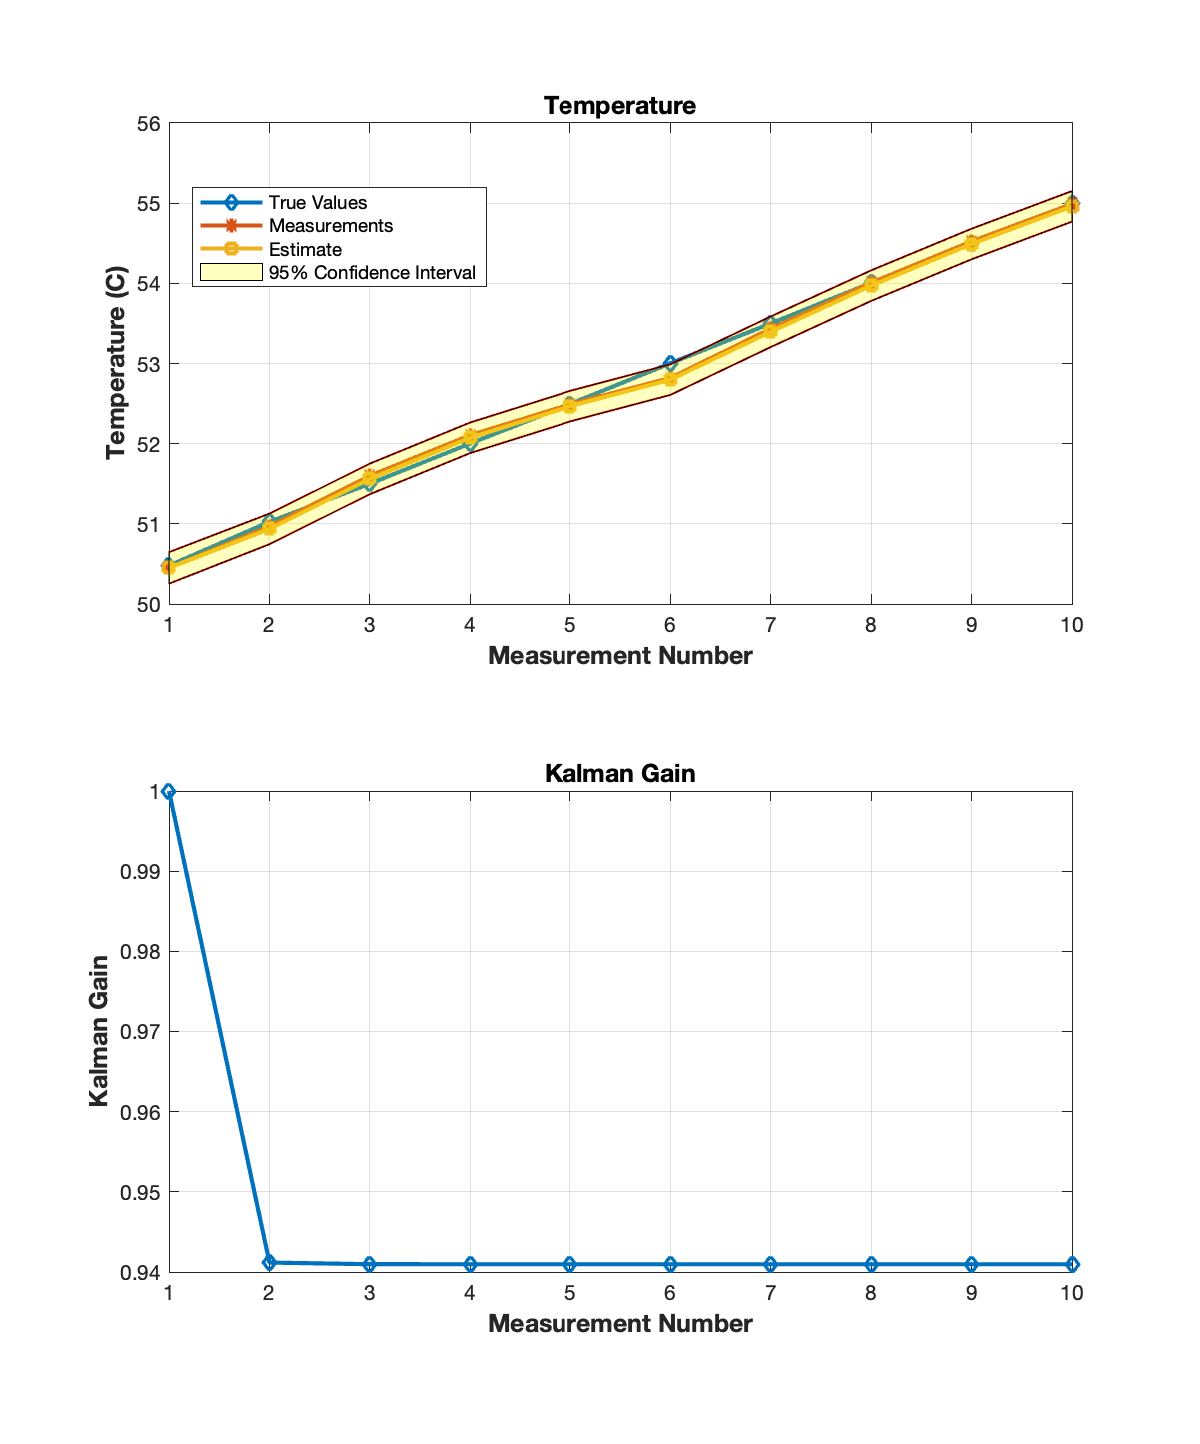
\includegraphics[trim={0 13cm 0 0},clip, width=0.5\linewidth]{Figures/Chapter1/ex8_KalmanFilter_ProcessNoise_II.eps}
\end{figure}

\item Assume that 100\% of the ground truth is within the confidence intervals. Is it good?
Not necessarily. Your KF estimates uncertainty is too high. You can achieve lower uncertainty estimates without compromising the confidence level.
\end{itemize}
    
\end{columns}
\end{frame}